Modern IDEs provide many useful code navigation facilities, for instance
allowing users to jump from a call site to the declaration of the called
function, or to find all the call sites of a particular function definition.
The reliability of such features is contingent on the availability of accurate
call graph information. However, \matlab's dynamic typing and dynamic features
complicate the problem of statically computing a precise call graph.

Previous work on \matlab call graph construction operated on a \matlab subset,
carefully ruling out those features which aren't amenable to static analysis,
with the ultimate goal of compiling \matlab to a statically typed language such
as \fortran or \xten \cite{Tamer}. As we mean to support regular \matlab
development, carving out such a subset is not an acceptable approach.

In this chapter, we present our approach to computing an accurate call graph
for arbitrary \matlab code. Rather than relying on static analysis, we extract
this information dynamically, by instrumenting the input programs and tracing
their actual execution on a \matlab implementation. This allows us to provide
precise code navigation even in the presence of features that have
traditionally been hard to reason about statically, such as calls to
\code{eval}. This precision comes at the cost of soundness, as the computed
call graphs are correct only with respect to a set of recorded program runs,
and some extra work for the programmer, whose responsibility it becomes to
provide entry points into the project that cover enough code to be useful.

\section{\matlab features complicating static call graph computation} \label{sec:MatlabLookup}

\matlab supports a limited form of function overloading or specialization. In
particular, it has a notion of \emph{superior} and \emph{inferior} types. While
the precise rules governing this relation are not documented anywhere, Dubrau
and Hendren, after exhaustively exercising each case, produced a diagram
(reproduced in \figref{fig:BuiltinClassRelationships}) describing the superior
and inferior relationships between the different builtin types \cite{Tamer}.
This relation is not a total ordering, as, for example, a given integer type is
neither superior nor inferior to the other integer types.

\begin{figure}[htbp]
\begin{center}
\includegraphics[width=5.2in]{figures/builtinClassRelationships.eps}
\caption{Superior/inferior type relationships for \matlab. An arrow points from
$a$ to $b$ if $a$ is superior to $b$.}
\label{fig:BuiltinClassRelationships}
\end{center}
\end{figure}

When a function call is evaluated, the arguments are evaluated first, and their
types influence the function lookup. In particular, \matlab identifies the most
superior argument type -- preferring the type of the leftmost superior argument
in case there is not a unique superior type -- and uses this as the call site's
"dominant type", say \code{char}. Then, a function defined in any directory
named \code{@char/} on \matlab's path will have priority over other
user-defined functions with the same name (with the exception of functions
nested inside the call site's enclosing function). Thus, in order to statically
compute a call graph in the presence of specialized functions, we need to carry
out type inference analysis to approximate these lookup semantics.

Although \matlab's functions are not quite first-class, a special kind of
object called a function handle can be used as a reference to a function,
either named or anonymous. These handles can be stored in variables, as well as
passed and returned from functions. Thus, in order to statically compute a call
graph in the presence of function handles, interprocedural analysis is required
to track which variables might hold function handles, and also which functions
each of these might point to.

In addition to these more traditional challenges, \matlab supports many highly
dynamic features that complicate any form of static analysis. Among these are
the evaluation of arbitrary strings as code via calls to the \code{eval} family
of functions, and a function lookup mechanism that involves crawling the
filesystem at runtime -- starting from a current directory that can be changed
at runtime -- in search of applicable call targets. More attention is paid to
these in \chapref{chap:DynamicFeatureElimination}.

\section{Call graph tracing instrumentation}

Since static analysis of \matlab code is difficult and easily misled in the
presence of dynamic features, we rely on dynamic analysis to extract
information that is sufficiently precise for our needs. Denker et al.
\cite{AbstractionsForDynamicAnalysis} identify different approaches available
to dynamic analysis tool developers for gathering runtime data:

\begin{itemize}
\item \emph{Source code modification} and, relatedly, \emph{logging services}.
This is the approach we ultimately use, as we discuss later.
\item \emph{Bytecode modification} or \emph{instrumenting the virtual machine}.
This requires knowledge of the internals of the \matlab virtual machine, and as
the reference \matlab implementation is a proprietary closed-source black box,
this isn't an option for us.
\item \emph{Method wrappers}. This refers to some mechanism for introducing
code to be executed before, after, or instead of a function. Our particular
source-to-source transformation, described later, can be seen of an instance of
this technique.
\item \emph{Debuggers}. While the reference \matlab implementation does include
a debugger, we prefer not to couple ourselves too tightly to it, as it is not
under our control.
\end{itemize}

The most natural and portable approach is source code modification. We can
implement it using the infrastructure provided as part of the \mclab toolkit.

The high-level idea is to insert logging statements before every possible call
site, and at the start of every function or script. After executing the
transformed code, we can post-process the logs and match up call sites with
their targets, since the target will follow the call in the log. We define a
unique identifier $identifier(n)$ for every call site and call target $n$; this
consists of the name of $n$ (the variable name if it's a variable, the function
name if it's a function definition, the script name if it's a script, and the
string \code{<lambda>} if it's an anonymous function expression), the file
it's contained in and its position (line and column) within that file. This
format comes in handy when it comes to implementing navigation features in an
IDE, as these typically take a textual range (e.g. a mouse selection) as input.

The transformation depends on a few functions (listed in
\figref{Fig:CallgraphRuntime}) being available at runtime. The
\code{mclab\_callgraph\_init} and \code{mclab\_callgraph\_log} functions
are straightforward; the former takes a path to a log file, creates it and
makes a handle to it globally accessible, while the latter takes a string and
writes it to the file. \newline \code{mclab\_callgraph\_log\_then\_run} is more
complicated; it takes a string, a variable (which is possibly a function
handle) and a variable number of arguments. If the given variable is a function
handle (either a function handle expression, or a variable that contains a
function handle), then we log the string to the file, and in either case we
forward the arguments to the variable.

\begin{figure}[htbp]
\lstinputlisting{code/callgraph_runtime.m}
\caption{The runtime components of the callgraph tracer.}
\label{Fig:CallgraphRuntime}
\end{figure}

Assuming these runtime functions are available, we traverse the whole project
and perform the following transformations.

\begin{itemize}

\item For every function or script $f$, we insert a call to
  \code{mclab\_callgraph\_log} as the first statement, passing the string
  \code{enter} followed by $identifier(f)$.

\item For every anonymous function definition $f$, we replace the body $b$ of the
  anonymous function with a call to \code{mclab\_callgraph\_log\_then\_run},
  passing the string \code{enter} followed by $identifier(f)$ as the first
  argument, and the original expression $b$ wrapped in an anonymous function
  expression taking no arguments as the second argument.

\item We replace every function call $n$ (as identified by the kind analysis)
  with a call to \code{mclab\_callgraph\_log\_then\_run}, passing the string
  \code{call} followed by $identifier(n)$ as the first argument, a handle to
  the target function as the second argument, and copies of the original
  arguments as the rest of the arguments.

  One caveat here is that there can be functions whose return value
  depends on the current execution context. For instance, \code{nargin} and
  \code{nargout} are builtin functions that return the number of input and
  output parameters passed to the current function. If we call these functions
  inside \code{mclab\_callgraph\_log\_then\_run} instead of the original
  function, they won't necessarily return the same value. As such, we avoid
  instrumenting calls to these functions, among other reflective functions such
  as \code{narginchk} and \code{inputname}. This doesn't really impact our
  precision, since these functions just return values, and can't for example
  call back into application code.

\item While the kind analysis distinguishes between function calls and variable
  accesses, it doesn't distinguish among the latter between array accesses and
  function handle invocations. In order to accurately trace control flow through
  function handles, we also instrument variable accesses in the same way as for
  function calls, only rather than passing in a function handle expression as
  the second argument, we just pass in the variable. At runtime,
  \code{mclab\_callgraph\_log\_then\_run} makes use of \matlab's reflective
  features to identify function handles, and only logs the call event in those
  cases. One small detail here is that an array access might have a colon
  literal as one of its arguments, and passing it to a function instead will
  cause \matlab to generate an error at runtime. In order for the
  transformation to be correct, we go through and replace any colon literals
  with colon string literals.

\end{itemize}

Finally, in order to trigger a tracing execution, an entry point is needed --
that is, a piece of code that will attempt to exercise as much of the subject
code as possible. This is handed off to the tracing machinery, which will first
instrument the project as described (in a temporary folder), create a temporary
file to hold the trace, and invoke \matlab, first calling
\code{mclab\_callgraph\_init} with the path to the log file, and then the
entry point. Once the execution is over, the trace is processed, and call
graph edges are identified by looking for \code{call} events that are
immediately followed by an \code{enter} event.

\figref{Fig:CallgraphBefore}, \figref{Fig:CallgraphAfter},
\figref{Fig:CallgraphTrace} and \figref{Fig:Callgraph} together show an
end-to-end example.

\begin{itemize}

\item \figref{Fig:CallgraphBefore} shows the application code.
  \code{for\_each\_file} recursively traverses a directory tree (using the
  builtin function \code{dir} as a primitive) and invokes a passed-in handler
  for each file with the given extension, making use of the helper functions
  \code{string\_ends\_with} and \code{is\_in} along the way. \code{code\_size}
  calls \code{for\_each\_file}, passing in a handle to the nested function
  \code{add\_size} as the handler. In \matlab, nested functions are closures,
  so that \code{add\_size} can read and write to the \code{total\_size}
  variable in the enclosing scope. In this way, \code{code\_size} adds up the
  sizes of all the m-files in the current directory.

\item \figref{Fig:CallgraphAfter} shows the same code after instrumentation
  (with all instances of the \code{mclab\_callgraph\_} prefix omitted for
  brevity).

\item \figref{Fig:CallgraphTrace} shows the generated trace, using an invocation
  of \code{code\_size()} as the entry point. Some events are omitted for brevity.

\item Finally, \figref{Fig:Callgraph} shows the call graph produced by
  processing the trace and matching up \code{call} and \code{enter} events.
  The call graph is in JSON format, mapping, for each covered call site, the
  call site's identifier to an array of function identifiers.

\end{itemize}

\begin{figure}[htbp]
\begin{minipage}{\linewidth}
  \lstinputlisting{code/callgraph-example/before/for_each_file.m}
\end{minipage}
\begin{minipage}{\linewidth}
  \lstinputlisting{code/callgraph-example/before/code_size.m}
\end{minipage}
\caption{The application code.}
\label{Fig:CallgraphBefore}
\end{figure}

\begin{figure}[htbp]
\begin{minipage}{\linewidth}
  \lstinputlisting{code/callgraph-example/after/for_each_file.m}
\end{minipage}
\begin{minipage}{\linewidth}
  \lstinputlisting{code/callgraph-example/after/code_size.m}
\end{minipage}
\caption{The same code after instrumentation.}
\label{Fig:CallgraphAfter}
\end{figure}

\begin{figure}[htbp]
\lstinputlisting[language={}]{code/callgraph-example/trace.txt}
\caption{The generated trace.}
\label{Fig:CallgraphTrace}
\end{figure}

\begin{figure}[htbp]
\lstinputlisting[language={}]{code/callgraph-example/graph.txt}
\caption{The generated call graph.}
\label{Fig:Callgraph}
\end{figure}

\section{Dealing with builtin and library functions} \label{sec:CallgraphBuiltins}

The abovementioned instrumentation can't be applied to \matlab builtin
functions. It could potentially be applied to library functions, assuming their
source code was available and they were written in \matlab and not native code.
That being said, if the goal is to enable useful code navigation features, then
instrumenting library functions is of dubious utility. In any case, during the
course of a profiling run, control flow is likely to be passed to a builtin or
otherwise uninstrumented function, which could then call back into the project
code, for instance via a passed-in function handle, a method call on a
passed-in object, or the use of \matlab's reflective features, possibly using
passed-in arguments to compute names of functions to call. Without taking
care to handle this correctly, then in the presence of such code, our approach
will be unsound, even with respect to the recorded execution.

As an illustrative example, consider the builtin function \code{arrayfun},
which takes a function handle $f$ and an array $a$ and applies $f$ to each
element in $a$, returning an array of the outputs, analogously to the
\code{map} function in functional languages. A call to \code{arrayfun} passing
in a handle to a user-defined function $f$ will manifest in the produced call
graph as an edge linking the call to \code{arrayfun} with $f$ directly, which
isn't quite correct. That information may still be useful for code navigation
purposes, with the understanding that we're tracking how control flow jumps
through application code, rather than focusing specifically on call sites and
their targets, but there again that's beyond the scope of a call graph
computation. A bigger problem occurs if $f$ itself calls a builtin function
$c$, as control would flow back to \code{arrayfun} which would invoke $f$
again, linking together the call to $c$ with $f$. Unlike the previous case,
this has no practical application, and is just wrong.

To preserve the soundness of our approach even in such cases, we rely on more
of \matlab's reflective features. In particular, the \code{functions} builtin
function allows us to inspect the contents of a function handle at runtime, and
determine which function it points to, the path to the file in which that
function was defined if applicable, and whether or not it's a builtin function.
Using this facility, we modify \code{mclab\_callgraph\_log\_then\_run} as shown
in \figref{Fig:LogThenRunBuiltin} to insert extra markers in the call trace in
order to distinguish calls to builtin functions. These markers are ignored by
the call graph construction step, but their presence in the trace separates
builtin call sites from user-defined function entrances, avoiding the addition
of the problematic edges.

\begin{figure}[htbp]
  \lstinputlisting{code/callgraph_builtins.m}
\caption{Code to handle builtins at runtime.}
\label{Fig:LogThenRunBuiltin}
\end{figure}

\section{Instrumentation performance overhead}

A priori, we expect the instrumented code to run at least an order of magnitude
or two slower than the original code, the main culprit being the wrapping of
every single function call or variable access with a call to an auxiliary
function. In order to get a sense of the magnitude of the overhead, we run some
benchmarks with and without instrumentation.

\subsection{Benchmarks}

We run our experiments on a set of 29 \matlab benchmarks. 23 of these are part
of the \mclab project's standard benchmark suite, which was collected from
various sources, including the FALCON and OTTER projects, Chalmers University
of Technology, the \matlab Central File Exchange, and the ACM CALGO library.
These benchmarks are mostly numerical algorithms, heavy on loops and array
reads and writes, and not so heavy on function calls or function handles. Most
\matlab code looks like this, so measuring and minimizing overhead on such code
is important. However, it's also important to evaluate our approach on code
where the tracing would reveal useful information. To that end, we also include
seven additional benchmarks in our suite. Six of these are numerical solvers, a
class of programs where it is common to operate on function handles. These are
the same benchmarks used by Lameed and Hendren to evaluate their work on
optimizing \code{feval} implementations \cite{OptimizingFeval}.

% TODO(isbadawi): Want a dynamic thing but get a static thing
These benchmarks are described briefly in
\tableref{tab:InstrumentationBenchmarks}. In
\tableref{tab:InstrumentationBenchmarksInstrumentable}, we include some simple
static metrics to help understand the following experimental results. Since
instrumenting a function call or array access adds an overhead proportional to
the number of times it is executed, we note, for each benchmark, how many calls
or accesses are instrumented (this is the first number in each column), and how
many of these are inside loops (this is the number in parentheses in each
column). Note that this is computed is a relatively simple-minded way, and
doesn't catch, for example, calls or accesses inside functions which are called
inside loops. Nevertheless, this can be an interesting metric. The "Naive"
column refers to the instrumentation described thus far. We then show how each
optimization described later in this section affects this metric (in other
words, how many expressions we are able to avoid instrumenting). These are the
"+ Prop", "- Builtins", and "+ Checks" columns; their specific meanings are
described in the following section.

\begin{table}
  \begin{tabular}{| l | p{10cm} |}
  \hline
  Name & Description \\  \hhline{|=|=|}
  adpt        & Adaptive quadrature via Simpson's rule \\ \hline
  arsim       & Simulates autoregressive model \\ \hline
  bbai        & Babai estimation algorithm \\ \hline
  bubble      & Bubble sort \\ \hline
  capr        & Computes capacitance of a transmission line via finite difference and Gauss-Seidel methods \\ \hline
  clos        & Calculates transitive closure of a directed graph \\ \hline
  create      & Simulated maximum likelihood statistical regression \\ \hline
  crni        & Solves heat equation via Crank-Nicholson \\ \hline
  dich        & Solves Laplace's equation via Dirichlet \\ \hline
  diff        & Calculates diffraction pattern of monochromatic light \\ \hline
  fdtd        & Applies finite-difference time domain technique \\ \hline
  fft         & Computes discrete fast Fourier transform on complex data \\ \hline
  fiff        & Calculates finite difference solution to wave equation \\ \hline
  lgdr        & Calculates derivatives of Legendre polynomials \\ \hline
  mbrt        & Computes Mandelbrot sets \\ \hline
  mcpi        & Computes $\pi$ via Monte Carlo method \\ \hline
  nb1d        & Simulates 1-dimensional n-body problem \\ \hline
  nb3d        & Simulates 3-dimensional n-body problem \\ \hline
  numprime    & Sieve of Eratosthenes \\ \hline
  optstop     & Solves optimal stopping problem \\ \hline
  quadrature  & Integrates function via quadrature \\ \hline
  scra        & Computes reduced-rank approximation of matrix \\ \hline
  spqr        & Computes semi-pivoted QR decomposition of matrix \\ \hhline{|=|=|}
  bisect      & Finds root of scalar function via bisection method \\ \hline
  gaussQuad   & Composite Gauss-Legendre quadrature \\ \hline
  newton      & Finds root of scalar function via Newton's method \\ \hline
  odeEuler    & Integrates first order ODE via Euler's method \\\hline
  odeMidpt    & Integrates first order ODE via midpoint method \\ \hline
  odeRK4      & Integrates first order ODE via Runge-Kutta \\ \hline
  sim\_anl    & Minimizes function via simulated annealing \\ \hline
\end{tabular}
\caption{Call graph instrumentation benchmarks.}
\label{tab:InstrumentationBenchmarks}
\end{table}

\begin{table}
\centering
  \begin{tabular}{| l | l | l | l | l | l |}
  \hline
  Name & Naive & + Prop & - Builtins & + Checks \\ \hhline{|=|=|=|=|=|}
  adpt        & 31 (21) & 15 (8) & 1 (1) & 1 (1) \\ \hline
  arsim       & 19 (9) & 12 (3) & 2 (2) & 1 (1) \\ \hline
  bbai        & 13 (8) & 13 (8) & 7 (5) & 2 (2) \\ \hline
  bubble      & 7 (4) & 6 (3) & 4 (3) & 1 (0) \\ \hline
  capr        & 37 (29) & 19 (11) & 12 (10) & 5 (3) \\ \hline
  clos        & 2 (1) & 2 (1) & 1 (1) & 1 (1) \\ \hline
  create      & 86 (79) & 66 (59) & 48 (48) & 45 (45) \\ \hline
  crni        & 25 (19) & 18 (12) & 10 (8) & 2 (2) \\ \hline
  dich        & 25 (9) & 11 (3) & 1 (1) & 1 (1)  \\ \hline
  diff        & 14 (10) & 14 (10) & 1 (1) & 1 (1) \\ \hline
  fdtd        & 39 (30) & 9 (0) & 1 (0) & 1 (0) \\ \hline
  fft         & 17 (14) & 10 (7) & 6 (5) & 1 (0) \\ \hline
  fiff        & 22 (21) & 18 (17) & 1 (1) & 1 (1) \\ \hline
  lgdr        & 21 (15) & 12 (6) & 3 (3) & 3 (3) \\ \hline
  mbrt        & 11 (3) & 11 (3) & 2 (1) & 2 (1) \\ \hline
  mcpi        & 3 (2) & 3 (2) & 1 (0) & 1 (0) \\ \hline
  nb1d        & 26 (12) & 25 (11) & 9 (4) & 5 (0) \\ \hline
  nb3d        & 35 (20) & 20 (7) & 6 (5) & 3 (0) \\ \hline
  numprime    & 3 (2) & 3 (2) & 1 (0) & 1 (0) \\ \hline
  optstop     & 15 (14) & 9 (8) & 6 (5) & 6 (5) \\ \hline
  quadrature  & 2 (1) & 2 (1) & 2 (1) & 2 (1)\\ \hline
  scra        & 48 (35) & 40 (27) & 25 (21) & 17 (13) \\ \hline
  spqr        & 48 (35) & 35 (27) & 21 (21) & 13 (13) \\ \hhline{|=|=|=|=|=|}
  bisect      & 31 (7) & 31 (7) & 6 (2) & 4 (2) \\ \hline
  gaussQuad   & 53 (4) & 18 (2) & 4 (1) & 4 (1) \\ \hline
  newton      & 16 (5) & 16 (5) & 3 (2) & 3 (2) \\ \hline
  odeEuler    & 7 (4) & 4 (1) & 2 (1) & 2 (1) \\\hline
  odeMidpt    & 10 (7) & 5 (2) & 3 (2) & 3 (2) \\ \hline
  odeRK4      & 7 (4) & 7 (4) & 5 (4) & 5 (4) \\ \hline
  sim\_anl    & 19 (8) & 12 (8) & 4 (2) & 4 (2) \\ \hline
\end{tabular}
\caption{Instrumentable expressions in each benchmark.}
\label{tab:InstrumentationBenchmarksInstrumentable}
\end{table}

\subsection{Results}

The results are shown in \tableref{tab:InstrumentationResults}. All the
programs were executed on a machine with an Intel\textregistered \,
Core\texttrademark \, i7 CPU @ 2.4 GHz and 8 GB of memory, running OS X 10.10,
using \matlab version R2014b. For each benchmark, we show the running times of
the original code in seconds, and the slowdown of each instrumented version
relative to the original code. The columns refer to the same versions as in
\tableref{tab:InstrumentationBenchmarksInstrumentable}, and the specific
meaning of the "Better runtime" is given in the following section.

For the naive instrumentation described thus far, we see that the slowdown can
be extreme for some benchmarks, with six of the benchmarks (capr, carni, dich,
diff, fiff and mbrt) undergoing a three order of magnitude slowdown. All of
these in the numerical category, and can be optimized. The functional
benchmarks all see a slowdown between one and two orders of magnitude. While
we're able to optimize them slightly, they tend to stay within the same order
of magnitude.

\begin{table}
\begin{tabular}{| l || l || l | l | l | l | l |}
  \hline
  Benchmark & Original & Naive & + Prop & - Builtins & + Checks & Better runtime \\ \hline
            & \multicolumn{1}{c||}{(s)} & \multicolumn{5}{c|}{Slowdowns} \\ \hhline{|=||=||=|=|=|=|=|}
  adpt        & 0.994 & 96.1 & 73.6 & 1.03 & 1.15 & 1.06    \\ \hline
  arsim       & 0.252 & 4.09 & 2.78 & 1.03 & 1.03 & 1.01    \\ \hline
  bbai        & 0.112 & 1.09 & 1.10 & 1.06 & 1.05 & 1.09    \\ \hline
  bubble      & 0.003 & 3.11 & 3.12 & 2.74 & 3.79 & 3.15    \\ \hline
  capr        & 10.7  & 1570 & 267 & 267 & 3.72 & 3.16      \\ \hline
  clos        & 0.358 & 1.08 & 0.99 & 1.01 & 1.07 & 1.01    \\ \hline
  create      & 0.033 & 2.36 & 2.62 & 1.49 & 1.63 & 1.78    \\ \hline
  crni        & 15.4  & 1040 & 470  & 485  & 1.07 & 1.17    \\ \hline
  dich        & 3.79  & 5340 & 2950 & 1.02 & 1.04 & 1.02    \\ \hline
  diff        & 1.24  & 1690 & 1660 & 1.02 & 1.05 & 0.98    \\ \hline
  fdtd        & 1.11  & 2.82 & 1.08 & 1.05 & 1.07 & 1.03    \\ \hline
  fft         & 1.95  & 283  & 145  & 144  & 2.54 & 2.11    \\ \hline
  fiff        & 4.83  & 2190 & 18.1 & 0.942& 0.922& 0.998   \\ \hline
  lgdr        & 0.014 & 3.29 & 2.53 & 1.87 & 1.87 & 1.69    \\ \hline
  mbrt        & 2.08  & 1490 & 1500 & 4.17 & 4.28 & 4.05    \\ \hline
  mcpi        & 0.007 & 2.96 & 2.97 & 2.08 & 1.95 & 2.12    \\ \hline
  nb1d        & 8.74  & 6.64 & 6.77 & 2.09 & 1.03 & 0.96    \\ \hline
  nb3d        & 0.737 & 2.85 & 2.09 & 1.14 & 1.03 & 1.03    \\ \hline
  numprime    & 0.005 & 2.31 & 2.36 & 2.72 & 2.70 & 2.78    \\ \hline
  optstop     & 0.048 & 2.46 & 2.48 & 1.59 & 1.81 & 2.35    \\ \hline
  quadrature  & 0.004 & 3.25 & 3.24 & 3.24 & 3.32 & 3.56    \\ \hline
  scra        & 0.134 & 1.42 & 1.35 & 1.14 & 1.12 & 1.14    \\ \hline
  spqr        & 0.119 & 1.38 & 1.28 & 1.09 & 1.15 & 1.15    \\ \hhline{|=||=||=|=|=|=|=|}
  bisect      & 0.761 & 61.3 & 60.8 & 24.1 & 22.9 & 17.9    \\ \hline
  gaussQuad   & 1.63  & 26.1 & 24.6 & 13.8 & 14.0 & 10.2    \\ \hline
  newton      & 1.26  & 42.1 & 41.7 & 22.5 & 22.4 & 16.3    \\ \hline
  odeEuler    & 0.519 & 814  & 686  & 696  & 677  & 580     \\ \hline
  odeMidpt    & 0.553 & 717  & 628  & 684  & 658  & 510     \\ \hline
  odeRK4      & 0.478 & 710  & 624  & 619  & 641  & 475     \\ \hline
  sim\_anl    & 0.682 & 61.6 & 56.2 & 18.6 & 18.6 & 13.9    \\ \hhline{|=||=||=|=|=|=|=|}
  Geometric mean & & 32.0 & 21.8 & 6.50 & 4.00 & 3.72 \\ \hline
\end{tabular}
\caption{Running times of the instrumented code with different optimizations
enabled.}
\label{tab:InstrumentationResults}
\end{table}

\section{Minimizing overhead}

The bulk of the runtime overhead of our approach stems from instrumenting each
function call and variable access, which is ultimately caused by our inability
to precisely distinguish arrays from function handles statically. Yet arrays
are apt to be much more common than function handles, so that the cost of
instrumenting each array access is disproportionate relative to the benefit.
Thus, we apply a few different techniques to try and minimize the amount of
array accesses that require instrumentation.

\subsection{Handle propagation analysis}

While the \mclab toolkit doesn't provide any facilities for performing
interprocedural static analysis on arbitrary \matlab code, we can still track
the flow of function handles through a single function. For each use of a
variable, we can estimate whether the variable holds only data, or a function
handle, or possibly a complex data structure with a mix of data and handles.
Where we're able to determine that a variable is definitely an array containing
only data, we can avoid instrumenting it. Some prior work had been done in this
direction inside the \mclab framework in the form of an intraprocedural
\emph{handle propagation analysis} -- work which we formalized and whose
implementation we completed.

The handle propagation analysis aims to compute, at each program point, which
variable possibly contain function handles. It's common to characterize
\matlab as a language where everything is a matrix -- even a scalar value is
actually a 1x1 matrix. Function handles, however, are not matrices. Broadly,
we distinguish between handles and structured data such as arrays, structs
or cell arrays. Then among these two categories we make some further
distinctions. In particular, the analysis deals with abstract values defined
as follows.

\begin{itemize}
  \item A variable could contain a function handle created via a function
    handle expression \code{@f}, which simply creates a handle to named
    function \code{f}. If so, we associate with the variable the abstract value
    $NAMED(f)$, keeping track of the name it points to.
  \item A variable could contain a function handle created via an anonymous
    function \code{@(x) expr(x)}. If so, we associate with the variable the
    abstract value $ANON(n)$, where $n$ is a reference to the
    anonymous function node in the AST.
  \item A variable could contain a function handle we don't have further
    information about. Typically this would happen if it was assigned the
    result of a call to a builtin function known to return handles. In that
    case we associate with the variable the abstract value $HANDLE$,
    abbreviated as $H$.
  \item A variable could contain structured data (for example a cell array),
    every element of which is a function handle. If so, we associate with it
    the abstract value $DHO$ (data, handle only).
  \item A variable could contain structured data where the elements are known
    to definitely not be handles. If so, we associate with it the abstract
    value $DO$ (data only).
  \item A variable could contain structured data which is a mix of handles
    and data, or where we don't know anything about the content. If so, we
    associate with the variable the abstract value $DWH$ (data with handles).
\end{itemize}

In addition to these, we have $\top$ and $\bot$ values, where $\top$ is the
most general value, and $\bot$ means the value is as yet undefined. The handle
propagation analysis is an intraprocedural forward dataflow analysis. At each
program point, it associates with each variable name a single abstract value.
The merge operation is the join $\vee$ of the partial order illustrated in
\figref{fig:HandleLattice}.

\begin{figure}
\centering
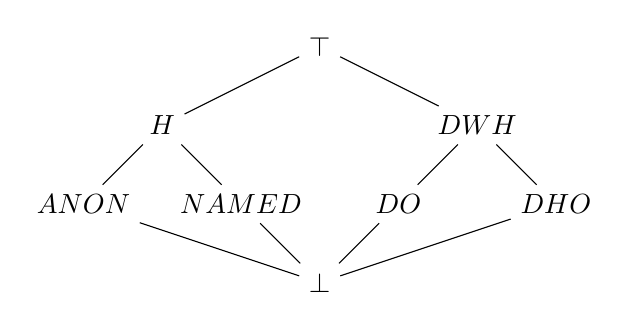
\begin{tikzpicture}
  \node (bot) at (0, 0) {$\bot$};
  \node (anon) at (-3, 1) {$ANON$};
  \node (named) at (-1, 1) {$NAMED$};
  \node (h) at (-2, 2) {$H$};
  \node (do) at (1, 1) {$DO$};
  \node (dho) at (3, 1) {$DHO$};
  \node (dwh) at (2, 2) {$DWH$};
  \node (top) at (0, 3) {$\top$};
  \draw [-] (bot) to (anon);
  \draw [-] (bot) to (named);
  \draw [-] (anon) to (h);
  \draw [-] (named) to (h);
  \draw [-] (bot) to (do);
  \draw [-] (bot) to (dho);
  \draw [-] (do) to (dwh);
  \draw [-] (dho) to (dwh);
  \draw [-] (h) to (top);
  \draw [-] (dwh) to (top);
\end{tikzpicture}
\caption{Handle propagation analysis abstract values.}
\label{fig:HandleLattice}
\end{figure}


The analysis operates on a regular \matlab AST, using \mcsaf, the \mclab
toolkit's static analysis framework. When we encounter an assignment statement
$S$, we first examine the top-level expression $E$ on the right hand side, and
compute from it an abstract value $gen(E)$. The rules for this are summarized in
\tableref{tab:HandleExprRules}, and explained in more detail below.

\begin{table}[htbp]
\begin{tabular}{l | l l r}
  Expression $E$ & Abstract value $gen(E)$ \\ \hline
  \code{@name}    & $NAMED(name)$ & & (1) \\ \hline
  \code{@(..)...} & $ANON(@(..)...)$ & & (2) \\ \hline

  $id$ & $in(id)$ & if $kind(id) = VAR$ & (3) \\
       & $info(id)$ & if $kind(id) = FN \wedge id \in info$ & (4) \\
       & $\top$ & if $kind(id) = FN \wedge id \not \in info$ & (5) \\ \hline

  $id(\dots)$ & $info(id)$ & if $kind(id) = FN \wedge id \in info$ & (6) \\
              & $\top$ & if $kind(id) = FN \wedge id \not \in info$ & (7) \\
              & $info(f)$ & if $in(id) = NAMED(f) \wedge f \in info$ & (8) \\
              & $\top$ & if $in(id) \in \lbrace H, ANON, NAMED \rbrace$ & (9) \\
              & $in(id)$ & otherwise & (10) \\ \hline

  $id\lbrace\dots\rbrace$ & $ DO $ & if $in(id) = DO$ & (11) \\
  $id.\cdots$ & $ H $ & if $in(id) = DHO$ & (12) \\
  $id.(\dots)$ & $\top$ & if $in(id) = DWH$ & (13) \\ \hline

  $\lbrace E_1, \dots, E_n \rbrace$ & $struct (\big\lbrace gen(E_1), \dots, gen(E_n) \big\rbrace)$ & & (14) \\
  $[ E_1, \dots, E_n ]$ & & \\ \hline
  any other expression & $DO$ & & (15) \\ \hline
\end{tabular}
\caption{Handle propagation analysis rules for computing $gen(E)$.}
\label{tab:HandleExprRules}
\end{table}

In \tableref{tab:HandleExprRules} and in what follows, we write $in(id)$ to
refer to the abstract value associated with the identifier $id$ in the in set
of $S$, and $kind(id)$ to refer to the kind analysis result for that identifier
(either FN or VAR, meaning the variable refers to a function or not,
respectively). While the analysis is intraprocedural over user-defined
functions, an attempt is made to avoid imprecision caused by calls to builtin
functions in the form of a table $info$, mapping, for a few hundred builtin
functions, their name to an abstract value representing their return value.

We consider the following cases for $E$.

\begin{itemize}

  \item $E$ is a function handle expression, or an anonymous function
    definition. In that case we simply generate the appropriate $NAMED$ or
    $ANON$ abstract value. This corresponds to rules (1) and (2).

  \item $E$ is a use of an identifier $id$. In \matlab, the parentheses can be
    omitted from a function call -- but not a function handle invocation -- if
    no arguments are passed. Thus $E$ is either a variable access, or a call to
    named function. The kind analysis is enough to distinguish between the two
    cases. If it's a variable, we simply propagate forward whatever information
    we had (rule (3)). If it's call to a function with has an entry in $info$,
    we use it (rule (4)). Otherwise, it's a call to an unknown function which
    might return anything, so we use $\top$ (rule (5)).

  \item $E$ is a parameterized expression $id(\dots)$. As in the previous case,
    $E$ could be a call to named function which we either have information
    about or not -- rules (6) and (7) in \tableref{tab:HandleExprRules} are
    identical to rules (4) and (5).

    Because of the parentheses, this might be a function handle invocation. If
    $in(id) = NAMED(f)$ -- that is, a handle to a named function $f$ -- and we
    have an entry for $f$ in $info$, then we can use it (rule (8)). If we don't
    know anything about $f$, or if $id$ contains a handle we don't know
    anything about, then we treat this as an arbitrary function call and use
    $\top$ (rule (9)).

    Otherwise, $id$ refers to a variable containing data -- either an array or
    a cell array (but not a struct, because structs can't be accessed with
    parentheses). Arrays in \matlab can't contain function handles. Cell arrays
    can contain handles, but indexing a cell array with parentheses (rather
    than braces) doesn't return the contained data directly, instead returning
    a set of cells. Thus in this case we can again simply propagate forward the
    information we already had for $id$ (rule (10)).

  \item $E$ could be a cell array indexing expression $id\lbrace\dots\rbrace$,
    or struct access expression $id.\cdots$ or $id.(\dots)$. We treat all of
    these cases the same way. If $id$ is known to only contain data ($DO$),
    then all of its elements only contain data, so we can use $DO$ again (rule
    (11)). If $id$ is known to only contain handles ($DHO$), then anything we
    pull out of it is necessarily a handle, so we can use $H$ (rule (12)).
    Otherwise, what we pull out might be data or a handle, and thus we use
    $\top$ (rule (13)).

  \item $E$ could be an array or cell array literal. For this case, we define a
    helper function $struct$ operating on abstract values (which we will reuse
    for the assignment cases later on). In particular, it takes in a set of
    abstract values and, interpreting them as the indvidual elements of an
    array or cell array $a$, returns an abstract value representing $a$ itself.
    If all the elements are data only, then the whole is data only. If the
    elements are all handles, or data containing handles, then the whole is
    data containing handles. Otherwise, the whole is data that might contain
    either data or handles. $struct$ is defined as follows.

\begin{align*}
struct(V) &= \begin{cases}
  DO & \text{if } V = \lbrace DO \rbrace \\
  DHO & \text{if } V \subseteq \lbrace H, NAMED, ANON, DHO \rbrace \\
  DWH & \text{otherwise} \\
\end{cases} \\
\end{align*}

    For this case, we traverse the literal and compute the abstract values for
    each of the constituent expressions, finally merging them together with
    $struct$ (rule (14)).

  \item $E$ could be any other expression. The ones we haven't considered yet
    include arithmetic and logical expressions, as well as numeric, string,
    colon and range literals. All of these either are or operate on data only
    (rule (15)).

\end{itemize}

\tableref{tab:HandleStmtRules} shows how $gen(E)$ is used to compute the new
abstract value for the variable being assigned to. In each case, $id$ is the
main identifier being assigned to in $S$. The out set of $S$ is the same as the
in set, with the value for $id$ replaced by value in the right hand column. We
distinguish just two cases for $S$.

\begin{itemize}

  \item $id$ is assigned to directly, as in $id = E$ for some expression $E$.
    In this case we simply take $gen(E)$ to be the new abstract value for $id$,
    replacing whatever was there before.

  \item $id$ is having one of its elements or fields assigned to. The idea here
    is that we know $id$ to be some sort of data structure, and only one of its
    elements is changing. For example, if $in(id) = DO$, and $E$ evaluates to a
    function handle, then $id$ is now a mix of data and handles.

    We model this succinctly by running $gen(E)$ through our $struct$ helper
    function from earlier. Given a single input value like this, $struct$ will
    simply coalesce handle values to $DHO$, and $\top$ to $DWH$, and otherwise
    return its input. If $in(id)$ is one of the data abstract values, then we
    just merge $in(id)$ with the value returned by $struct$. If $in(id) = \top$
    for whatever reason, then we still know that after $S$, $id$ will not be a
    handle, so we use $DWH$, the most general data value.
\end{itemize}

\begin{table}
\begin{tabular}{l | l l}
  Assignment & $out(id)$ & \\ \hline
  $id = E$ & $gen(E)$ & \\ \hline
  $id.\cdots = E$ & $in(id) \vee struct(\lbrace gen(E) \rbrace)$ & if $in(id) \in \lbrace DWH, DHO, DO \rbrace$ \\
  $id\lbrace\dots\rbrace = E$ & $DWH$ & otherwise \\
  $id.(\dots) = E$ & & \\
  $id(\dots) = E$ & & \\ \hline
\end{tabular}
\caption{Handle propagation analysis rules for assignments.}
\label{tab:HandleStmtRules}
\end{table}

% TODO(isbadawi): example here

% TODO(isbadawi): Maybe revisit this?
% Consider e.g.
% a = @abs;
% a = zeros(a(5));
% Contrived, but eh.
For our purposes, given a parameterized expression $id(\dots)$, we only need to
instrument it if $out(id) \in \lbrace NAMED, ANON, H, \top \rbrace$. We make
the decision based on the abstract value associated with the variable in the
statement's out set, rather than its in set. To see why, consider the function
in \figref{Fig:OutSetNotInSet}. Since \code{a} is a function parameter, we
conservatively assign it the value $\top$. Once it is assigned to on line 3, it
gets the value $DWH$, so we would know not to instrument it, but before that
statement, its value is still $\top$, so we would have to instrument it. If $a$
were a handle, however, then the assignment on line 3 would cause a runtime
error. By using the value in the out set, we can avoid over instrumenting in
these cases.

\begin{figure}[htbp]
\begin{lstlisting}[numbers=left]
function f(a)
  for i = 4:1000
    a(i) = a(i-1) + a(i-2) + a(i-3);
  end
end
\end{lstlisting}
\caption{A code snippet where a variable is used and assigned to in the same statement.}
\label{Fig:OutSetNotInSet}
\end{figure}

The "+ Prop" column in \tableref{tab:InstrumentationBenchmarksInstrumentable}
shows how many expressions remain instrumented with this enhancement applied,
and the corresponding column in \tableref{tab:InstrumentationResults} shows
the performance of the instrumented code as a slowdown relative to the
original uninstrumented code. In general the analysis is very effective,
weeding out many array accesses, and leading to big performance boosts; the
capr benchmark, for example, runs nearly an order of magnitude faster, going
from a 1578x slowdown in the naive version to a 293x slowdown.

\subsection{Avoiding builtin call instrumentation}

\matlab code tends to be fraught with calls to builtin functions, and
instrumenting these won't give much benefit, since we don't have access to
their source code. However, because \matlab builtin functions can be shadowed
by user-defined functions with the same name, or specialized via the mechanism
described in \secref{sec:MatlabLookup}, we can't necessarily tell statically
whether a given function call is a call to a builtin function. Because of this,
the naive instrumentation goes ahead and instruments every function call, even
if it likely is a call to a builtin.

While we can't statically determine the target of a function call to check
whether it's a builtin, we can examine the application's code, as well as any
library code it depends on, in order to gather a list $A$ of user-defined
functions whose names conflict with builtin functions. In \matlab, a function's
name is the name of the file it's defined in (less the extension), so this is
just a simple filesystem traversal. Then, during instrumentation, when we
encounter a potential call to a builtin function, we check whether the name of
function appears in $A$. If it doesn't, then we can safely avoid instrumenting
the call. One assumption here is that we have access to all the code the user
is apt to run; this is not unreasonable, given that the user is requesting a
call graph, and so is likely willing to provide all the relevant code.

We make a special exception for the builtin function \code{feval}, which is
often used to invoke function handles instead of the regular function call
syntax. There are two reasons for its prevalence. For one thing, in addition to
accepting function handles to invoke, \code{feval} also accepts names of
functions as strings, and it has become idiomatic in \matlab for library code
to offer similar interfaces -- accepting either handles or strings and
forwarding them to \code{feval} -- when a user-specified function is needed.
\code{feval} is also prevalent for historical reasons. Function handles were
added to the language with the release of \matlab 6 in 2000, but initially
could only be invoked via \code{feval}. Support for invoking function handles
with the regular function call syntax was not added until the release of
\matlab 7 in 2004. Given all this, we can almost view \code{feval} as an
alternative syntax for a function call. We therefore instrument all calls to
\code{feval}.

As as aside, in \secref{sec:CallgraphBuiltins}, we discussed the complications
caused by instrumenting calls to builtin functions. Even though we decide here
not to instrument direct calls to builtins, those complications still arise,
because function handles can point to builtin functions, and in those cases the
same problem traces -- with call events that don't have a corresponding enter
event -- can happen. Thus, the changes to the runtime described in that section
are still necessary.

The "- Builtins" column in
\tableref{tab:InstrumentationBenchmarksInstrumentable} shows how many
expressions remain instrumented with this enhancement applied (in addition to
the handle propagation analysis described in the previous section) and the
corresponding column in \tableref{tab:InstrumentationResults} shows the
performance of the instrumented code as a slowdown relative to the original
uninstrumented code. The effect of this optimizations depends on how heavily
the benchmark relied on builtin functions, but it is in general very effective,
in many cases (e.g. dich, diff) reducing the overhead to near 0.

\subsection{Checking type of function arguments at runtime}

Our instrumentation speculatively wraps each variable access in a function call
in case the variable is a function handle. A runtime check to determine whether
it is occurs inside this auxiliary function. This simplifies the
transformation, but is clearly wasteful if the variable turns out to be a plain
array variable, especially if the variable is accessed more than once. Since
\matlab is used a lot for numerical computations, \matlab code tends to be
heavy on loops, such that array variables are often accessed repeatedly,
magnifying the overhead. Intuitively, we should be able to check the type of a
given variable only once, and avoid instrumenting accesses to it at all if it's
not a function handle.

However, this presents a complication in terms of implementation complexity.
Wrapping each variable access in a function call is a very simple
transformation to make, as it just involves replacing an expression AST node
with another. If we start introducing conditionals, the transformation becomes
a lot more intrusive, since \matlab does not support any kind of conditional
expression (such as the ternary \code{\?:} operator in C-based languages), only
conditional statements. Thus, inserting checks at the right places while
preserving the order of operations requires destructuring the code into a kind
of three-address form.

The handle propagation analysis is precise enough in practice if we restrict
ourselves to a single function -- a lot of the imprecision occurs when arrays
are passed around as function parameters. As a simple middle ground, we create
two instrumented versions of each function. In the first version ($S$ for
slow), we seed the handle propagation analysis with the conservative assumption
that any of the function parameters might be a function handle (this is the
same assumption we've been using thus far). In the second ($F$ for fast), we
seed it with the assumption that all of the function parameters are definitely
just plain data arrays. We then instrument both versions independently.

If both versions are the same, then there's nothing to do. Otherwise, we
replace the body of the function with an if statement, with $S$ as the then
branch, and $F$ as the else branch. The condition checks at runtime, for each
input parameter $p$ with at least one use instrumented in $S$, whether $p$
is a function handle (using the \matlab builtin function \code{isa}).

The "+ Checks" column in \tableref{tab:InstrumentationBenchmarksInstrumentable}
shows how many expressions remain instrumented along the fast path where the
check reveals there are actually no handles, and the corresponding columns in
\tableref{tab:InstrumentationResults} shows the performance of the instrumented
code with these and all previous enhancements applied. For our more typical
\matlab benchmarks that are heavy on array operations, this drastically reduces
the overhead. For the benchmarks that do use function handles, the effect on
performance is predictably negligible.

\subsection{Optimized runtime functions}

The optimizations described thus far aim to reduce the number of expressions
requiring instrumentation. This helps tremendously on our numerical benchmarks,
where the call graphs are actually empty, or contain a single edge linking a
call from the benchmark's driver function to the benchmark itself; in these
cases, we can reduce the overhead to be negligible. For those expressions
where instrumentation is actually needed, however, we also investigate the
runtime overhead associated with each function call.

After some profiling on a long-running benchmark, we identify the following
bottlenecks.

\begin{itemize}

  \item Our runtime uses the \code{fprintf} functions to log call and enter
    events to a log file. It turns out that by default, \matlab's
    implementation of \code{fprintf} flushes the output buffer each time the
    function is called, so that each of these calls is actually hitting the
    filesystem. For builtin functions, this happens three times per call.

    In addition to the usual \code{'w'} and \code{'a'} writing modes,
    \matlab's \code{fopen} function also accepts \code{'W'} and \code{'A'},
    which behave similarly to their lowercase couterparts, except that the
    output buffer is not flushed until it either reaches capacity or the file
    is closed (via the \code{fclose} function). Simply making this one
    character change in the \code{mclab\_callgraph\_init} functions leads to
    a 1.5x speedup.

  \item Function calls in \matlab are quite expensive. The
    \code{mclab\_callgraph\_log\_then\_run} calls \code{mclab\_callgraph\_log}
    to do the writing -- inlining this call leads to significant performance
    boost.

\end{itemize}

The "Better runtime" column in \tableref{tab:InstrumentationResults} shows the
performance of the instrumented code with these enhancements applied.

\section{Related work}

Seeking to work around the difficulties posed by JavaScript's dynamic features,
Wei and Ryder \cite{TaintAnalysisForJavaScript} present a blended static and
dynamic analysis framework. The idea is to use an instrumented JavaScript
engine to execute tests covering the code we wish to analyze (the existence of
tests with sufficient coverage is assumed); this "dynamic phase" collects
information like the dynamic calling structure of the program, the types of
created objects, and any code that is dynamically loaded. A "static phase" then
uses the collected execution traces to build a call graph and guide static
analysis. This hybrid approach was found to have better performance and
accuracy than purely static approaches on selected benchmarks.

Motivated by the same problem of powering code navigation features in an IDE
setting, Feldthaus et al. present a static field-based flow analysis for
JavaScript \cite{ApproximateCallGraphsIDEServices}. In the face of JavaScript's
dynamism, they eschew soundness, instead focusing on the efficient construction
of approximate call graphs, which through empirical evaluation seem to be good
enough in practice.

Our handling of builtin functions was inspired by Ali and Lhot\'{a}k's work on
application-only call graph construction
\cite{ApplicationOnlyCallGraphConstruction}, in which they study the problem of
preserving the soundness of a Java call graph in the presence of unanalyzed
library code.
